\documentclass[12pt,a4paper, oneside]{book}
\usepackage{a4wide}
\usepackage[pdftex]{graphicx}
\usepackage{epstopdf}
\usepackage[american]{babel}
\usepackage{cite}
\usepackage{array}
\usepackage{theorem}
\usepackage{mathrsfs}
\usepackage{hvdashln}
\usepackage{arydshln}
\usepackage{amsmath,amsfonts,amssymb,bbm}
\usepackage{fancyhdr}
\usepackage{pstricks}
\usepackage{rotating}
\usepackage{courier}
\usepackage{hyperref}
\usepackage{placeins}
\usepackage{verbatim}
%\usepackage{multirow}

\definecolor{listinggray}{gray}{0.98}
\definecolor{lbcolor}{rgb}{0.98,0.98,0.98}
\usepackage{listings}
\lstset{
    fancyhdr,
	backgroundcolor=\color{lbcolor},
	tabsize=4,
	rulecolor=,
	language=matlab,
    basicstyle=\scriptsize\ttfamily,
    upquote=true,
    aboveskip={1.5\baselineskip},
    columns=fixed,
    showstringspaces=false,
    extendedchars=true,
    breaklines=true,
    prebreak = \raisebox{0ex}[0ex][0ex]{\ensuremath{\hookleftarrow}},
    frame=single,
    showtabs=false,
    showspaces=false,
    showstringspaces=false,
    identifierstyle=\ttfamily,
    keywordstyle=\color[rgb]{0,0,1},
    commentstyle=\color[rgb]{0.133,0.545,0.133},
    stringstyle=\color[rgb]{0.627,0.126,0.941},
}
\newcommand{\N}{\ensuremath{\mathbbm{N}}}
\newcommand{\Z}{\ensuremath{\mathbbm{Z}}}
\newcommand{\Q}{\ensuremath{\mathbbm{Q}}}
\newcommand{\R}{\ensuremath{\mathbbm{R}}}
\newcommand{\C}{\ensuremath{\mathbbm{C}}}
\newcommand{\rd}{\ensuremath{\mathrm{d}}}
\newcommand{\id}{\ensuremath{\,\rd}}
\newcommand{\HRule}{\rule{\linewidth}{0.5mm}}


%=============================
%fancy headings
\pagestyle{fancyplain}
\renewcommand{\chaptermark}[1]{\markboth{#1}{}}
\renewcommand{\sectionmark}[1]{\markright{\thesection\ #1}}
\lhead[\fancyplain{}{\nouppercase{\rmfamily\small\textbf\thepage}}]%
      {\fancyplain{}{\nouppercase{\rmfamily\small\textbf\rightmark}}}
\rhead[\fancyplain{}{\nouppercase{\rmfamily\small\textbf\leftmark}}]
      {\fancyplain{}{\nouppercase{\rmfamily\small\textbf\thepage}}}
\cfoot{}
%=============================

\newcommand{\dee}{\,\textrm{d}}
\newcommand{\mv}[1]{\boldsymbol{\mathsf{#1}}} % for matlab matrices and vectors
\newcommand{\pv}[1]{\boldsymbol{#1}} % for physical vectors (3 elements)

\newcommand{\courier}[1]{{\fontfamily{pcr}\selectfont #1}}
\newdimen\ptsize
\ptsize=12pt

\hdashlinewidth=2pt
\hdashlinegap=2pt

\renewcommand{\baselinestretch}{1.2}
\parindent=0pt

\setlength{\hoffset}{-5pt} \setlength{\oddsidemargin}{20pt}
\setlength{\evensidemargin}{-20pt}

\setlength{\parskip}{\baselineskip}

\begin{document}
\selectlanguage{american}
% \include{abstract4Paper}
\pagenumbering{roman}
% \thispagestyle{empty}
% $ $\\
% \begin{center}
% \Large \bf Scattering and absorption of radome\\[0.5cm]
% \small using method of equivalent dipole moment\\[1cm]
% \end{center}
% \begin{center}
% \normalsize \rm Author: Majid Naeem\\
% \normalsize \rm Manuscript version: 06 Oct. 2010
% \end{center}
% \newpage
% \thispagestyle{empty}
%\thispagestyle{empty}
%$ $\\
%\begin{center}
%\Large \bf Title of the MSc Project\\[6.1cm]
%\end{center}
%\newpage
\thispagestyle{empty}
$ $\\
\begin{center}
\Large \bf  Simulations of Dipole- and Array- Antenna in MATLAB\\[6.1cm]
\normalsize \rm
\\

%(interim report) \\[1cm]
%as part of mandatory clauses in \\fulfillment of Master's Degree from the \\
Chalmers University of Technology, Gothenburg, Sweden \\[1cm]
by \\[1cm]
\bf Marika Svensson\\
\bf Department of Signals and Systems \\[1cm]
\normalsize \rm
June 15, 2015
\end{center}
\newpage
\thispagestyle{empty}
\noindent%\large
Properties of Sparse Array Antennas / by \\ Marika Svensson. - Gothenburg : Chalmers University of Technology, 2015.\\

Copyright \copyright 2015 by Marika Svensson, Antenna Group, Signals and Systems Department, Chalmers University
of Technology, Gothenburg, Sweden; RUAG Space AB, Gotheburg, Sweden.\\[2ex]
This thesis is carried out under supervision of: \\
Dr. Johan Wettegren \\ \\
Examiner:\\
Prof. Marianna Ivashina\\ \\
Co-Supervisors: \\
Dr. Rob Maaskant \\
Carlo Bencivenni \\ \\%[2.5cm]
Keywords: antenna arrays / irregular array antennas / ... / ... \\
Subject headings: antenna arrays / irregular array antennas / ... / ... \\
\mbox{$ $ \hspace{1cm}} \\[3ex]
Technical Report No. 2015:xx \\
Antenna Group, Department of Signals \& Systems \\
Chalmers University of Technology, \\
SE-41296, Gothenburg, Sweden. \\
Telephone: +46 31 772 1000 \\ \\
% \normalsize A catalogue record is available from the Chalmers
% University of Technology Library\\[2ex]
Cover design:  Marika Svensson\\
Press: Chalmers Reproservice, G\"oteborg \\[2ex]
The work presented in this thesis has been financed by ...; 
and has been performed at ...

\newpage
\thispagestyle{empty}
$ $\\
\begin{center}
\Large \bf Abstract
\end{center}

\emph{In this report  two types of antennas were simulated in MATLAB. Initially  a horizontal dipole antenna was investigated by computing the far field function, the radiated power and lastly the far field patterns in the E- and H-plane. }\\

\emph{Then an irregularly spaced array antenna was investigated. First the far field was computed as a function of antenna positions and excitation current. Then the  excitation current was computed as a function of scanning angles and array element positions. Lastly an equispaced array antenna was considered. The radiation pattern were computed for the H plane and broadside with different intermediate spacing d. }

%\emph{The result of from the simulations corresponded well/badly with expected theoretical results.}
\tableofcontents
\cleardoublepage
\clearpage
% \include{Symbols}
% \thispagestyle{plain}
%\include{Acronyms}
\pagenumbering{arabic}
%\chapter{Micro Project}\label{Chap1}
\section{Objectives}
A one-week project with the aim to assess the MATLAB programming experience and the antenna array knowledge of the MSc student candidate.

\section{Tasks}
\begin{enumerate}
\item Write a MATLAB function that computes the far field function of a short electrical dipole antenna placed $\lambda/4$ above a PEC ground plane.
\\Input parameters: $\theta$ and $\phi$ observation angles, excitation current $I$.
\\Output parameters: vector far-field function $\pv{G}(\theta,\phi)=G_\theta(\theta,\phi)\pv{\hat{\theta}}+G_\phi(\theta,\phi)\pv{\hat{\phi}}$.
\\ \emph{Hint: cf. chapter 5.1.13}
\item Write a MATLAB function that computes the total radiated power through numerical integration.
\\Input parameters: far-field function $\pv{G}(\theta,\phi)$.
\\Output parameters: the radiated power $P_{\text{rad}}$.
\\\emph{Hint: cf. chapter 2.3.8}
\item Write a MATLAB function that plots the normalized far-field pattern in dBi for the E- and H-plane cuts.
\\Input parameters: $\pv{G}(\theta,\phi)$, observation angles.
\\Output parameters: a plot of the power pattern E- and H-plane cuts in dBi.
\\\emph{Hint: for the normalization in dBi you will need $P_{\text{rad}}$, cf. chapter 2.3.9}
\item Write a MATLAB function that computes the far-field function of an $N$-element dipole antenna array.
\\ Input parameters: matrix with antenna positions
\begin{align}
\left[
\begin{matrix}
x_1 & y_1 & z_1\\
x_2 & y_2 & z_2\\
 & \vdots & \\
x_N & y_N & z_N
\end{matrix}
\right]
\end{align}
vector of excitation currents $[I_1, I_2, \ldots, I_N]$.
\\ Output parameters: $\pv{G}(\theta,\phi)$ for the entire array beam.
\\ \emph{Hint: cf. chapter 10.1.1, 10.3.1}
\item Write a MATLAB function that computes the phased array excitation vector in order to scan the array to a certain direction.
\\Input parameters: scan angle $(\theta_0,\phi_0)$.
\\Output parameters: excitation vector $[I_1, I_2, \ldots, I_N]$.
\\ \emph{Hint: cf. chapter 10.1.4,10.3.3}
\item Using the pattern plotting function of point 3, observe the array pattern of a uniform linear array of 5 dipoles in a side-by-side configuration when: 
\begin{itemize}
\item the beam is scanned scanned in the H-plane, element spacing is $d = 2/3\lambda$.
\item the beam is pointed broadside, element spacing is swept from $d = \lambda/4$ to $4\lambda$
\end{itemize}
\end{enumerate}

\section{Report}\label{Rep}
Report the above results in this LaTeX document (this MSc template report): present it in a narrative way following the above points 1-6, while including and describing the results/plots, include the MATLAB scripts, and present it orally. The work is possible to finish in one week, if not, try to complete as many items as possible.

\section{References}\label{Ref}
\begin{itemize}
\item Foundations of Antennas: A Unified Approach, Per-Simon Kildal, 2014
\item MATLAB, The MathWorks Inc., Natick, MA, 200
\end{itemize}

\chapter*{Introduction}
\label{chapter:introduction}

The purpose of this report was to evaluate the knowledge of antenna simulations and general competence in MATLAB.  This was illustrated by computing the far field functions $\mathbf{G}(\theta, \phi)$, radiated power $P_{rad}$, radiation patterns, far field patterns, array factor patterns and excitation currents $\{I_n\}$ of different types of antennas in MATLAB. 

Two kinds of antennas were considered. In chapters \ref{chapter:task1}-\ref{chapter:task3} a horizontal dipole antenna was simulated in MATLAB where first the far field of the dipole antenna was computed as a function of observation angles and the excitation current. Then the total radiated power was computed as a function of the far field, then the far field patterns  and co polar radiation patterns evaluated as a function of the far field and observation angles in the E- ad H-plane were computed and plotted.

 In chapters \ref{chapter:task4}- \ref{chapter:task6} the second type of antenna to be considered was array antennas. First the far field function was computed for an irregular array antenna as a function of element position and excitation current. Then the excitation current was computed, as a function of scanning angles and element positions for an irregularly spaced array antenna. The amplitude of this current was set to unity. Lastly an equispaced array was considered and the far field, the radiation patterns were computed in the H-plane and broadside as a function of the far field of the array antenna and observation angles. 
 
 I chapter \ref{chapter:discussion} the results from the dipole and array antennas will be discussed, in appendix A the complete code written in MATLAB may be viewed by the reader.  
\chapter{Task 1} 
\label{chapter:task1}
In this section a horizontal dipole was simulated with MATLAB. The far field function of the dipole was computed as a function of the angles $\theta$, $\phi$ and excitation current I, which was set to unity. 

We will begin by presenting the theory of the dipole antenna and the far field region in electromagnetic theory. Then we will proceed with presenting the results generated from the MATLAB simulations.  


\section{Theory}
% Far field region
Antenna theory can be greatly simplified be the fact that the fields and different quantities are considered in the far field region only, which is the region where $r > 2D^2/\lambda$. This means that many complicated integrals, Lagrange polynomials, sums  etc. are instead approximated.

Begin by considering the electric field at a point in space $\mathbf{r} = \mathbf{R} + \mathbf{r_0}$ where the origin is set to be $\mathbf{r_0}$ for this coordinate system. The electric field can be considered as a function of $R, \theta, \phi$, i.e. 
\begin{equation}
E(r, \theta, \phi) = E(R, \theta, \phi).
\end{equation}  
and  the far field function times an exponent (which is the electrical field) can be rewritten as 
\begin{align}
\label{elField}
&G( \theta, \phi) \frac{e^{-jkr}}{r} = G'( \theta, \phi) \frac{e^{-jkR}}{R} \approx \\
&\approx G( \theta, \phi) e^{-jk(r-R)}\frac{e^{-jkR}}{R} =  G( \theta, \phi) e^{-jk(\mathbf{r}_o\cdot \hat{r})}\frac{e^{-jkR}}{R}
\end{align}  
where R is the distance $|\mathbf{r} - \mathbf{r}_0|$. In order to do the steps the Fraunhofer approximations in the far field were used,
\begin{equation}
\begin{cases}
& \frac{1}{r} \approx \frac{1}{R} \\
& r \approx R + \mathbf{r}_0\cdot \hat{r}.
\end{cases}
\end{equation}
It is the obvious that the far field can be written as
\begin{equation}
\mathbf{G}_A(\theta, \phi) = \mathbf{G}(\theta, \phi)e^{jk\mathbf{r}_A\cdot \hat{r}} 
\end{equation}
in a space position $\mathbf{r}_A$.
% Mor thoery? !

% Dipole
Consider now a dipole which has a $\hat{I}$ direction, a corresponding current density to this dipole will be 
\begin{equation}
\mathbf{J}_l(l')= I_0 j(l')\hat{I}
\end{equation}
where $I_0$ is the magnitude of the current and j is set to 
\begin{equation}
j(l) = \frac{sin\left(k\left( \frac{l}{2}- |z'|\right)\right)}{sin(kl/2)}.
\end{equation}
The electric field for a dipole may be written as a 
\begin{equation}
\mathbf{E}_d (\hat{r})= \frac{e^{-jkr}}{r}\mathbf{G}_d(\hat{r})
\end{equation}
which is a similar to to equation \eqref{elField} but with a far field which can be written as 
\begin{equation}
\begin{cases}
&  {G}_d(\hat{r}) = \eta I_0C_k[\hat{I}-(\hat{I}\cdot \hat{r})\cdot\hat{r} ]\hat{j}(l\hat{I}\cdot\hat{r}) \\
& \hat{j} = \int_{-l/2}^{l/2}j(l')e^{klj'\hat{I}\cdot\hat{r}} \approx l/2 \text{  if short dipole}
\end{cases}
\end{equation}
% More explination..?!

%Horizontal dipole
Consider finally a horizontal dipole, which is  a dipole with its direction in the y direction. This gives the expressions 
\begin{align}
& \hat{I} = \hat{y} \\
& \hat{I} \cdot \hat{r} = sin\theta sin\phi \\ \label{IrRes}
& \hat{I} -(\hat{I} \cdot \hat{r})\hat{r} = cos\theta sin\phi \hat{\theta} + cos\phi \hat{\phi}. 
\end{align}
The equations above can be understood be considering the spherical coordinates 
\begin{equation}
\begin{cases}
&\hat{x} = sin\theta cos\phi \hat{\theta} + cos\theta cos\phi \hat{\phi} - sin\theta \hat{r} \\
&\hat{y} = sin\theta sin\phi \hat{\theta} + cos\theta sin\phi \hat{\phi} - sin\phi \hat{r} \\
&\hat{z} = -sin\theta  \hat{\theta} - cos\theta \hat{r},
\end{cases}
\end{equation}
It can easily be seen that \eqref{IrRes} indeed holds.



The far field function  for a dipole of length l, sitting at height h can then be written as 
\begin{align}
&\mathbf{G}(\theta, \phi) = C_k\eta I_0 \hat{j}(k\hat{I} \cdot \hat{r})(cos\theta sin\phi \hat{\theta} + cos\phi \hat{\phi} )(e^{jkhcos\theta} -e^{-jkhcos\theta}) \\
& \approx C_k\eta I_0 \hat{j}(k\hat{I} \cdot \hat{r})(cos\theta sin\phi \hat{\theta} + cos\phi \hat{\phi} )(sin(khcos(\theta))). \\
\end{align}
If the dipole is considered to be short  $\hat{j} \approx l/2 $, so the far field function can be described according to  
\begin{equation}
\mathbf{G}(\theta, \phi) = G_{\theta}\hat{\theta} + G_{\phi}\hat{\phi},
\end{equation}
where the $\theta$ and $\phi$ parts of $\mathbf{G}$ are given by the expression

\begin{equation}
G_{\theta} = G_{\theta}(\theta, \phi) = Acos(\theta)sin(\phi)2jsin(khcos(\theta)))
\end{equation}
and 
\begin{equation}
G_{\phi} = G_{\phi}(\theta, \phi) = Acos(\phi)2jsin(khcos(\theta))).
\end{equation} 
The constant A is defined as 
\begin{equation}
A = C_k\eta I_0 l/2
\end{equation} 
with 
\begin{equation}
\begin{cases}
& C_k = -jk/4\pi \\
& \eta \approx 120 \pi [\Omega] \\
& k = \frac{2*pi}{\lambda} \\
& h = \frac{\lambda}{4}\\
& I_0 = \text{incident current}
 \end{cases}
\end{equation}\cite{kildal2000foundations}

\section{Results}
The code for task 1 can be viewed in appendix \ref{section:task1.m}, where the length of the dipole was chosen to be 0.1 $\lambda$ and I to be 1 A in order to get numerical results. 

The $\theta$ part of the far field function can be viewed in figure \ref{task1:Gth} as a function of the angles $\theta$ and $\phi$. 

\begin{figure}[h]
\centering
\includegraphics[scale=0.4]{/Users/marikasvensson/Documents/MATLAB/MicroProject/finished/task1/Gth.png}
\caption{This figure shows $G_\theta$ as a function of $\theta$ and $\phi$}
\label{task1:Gth}
\end{figure}


The $\phi$ part of the far field function can be viewed in figure \ref{task1:Gphi} as a function of the angles $\theta$ and $\phi$.


\begin{figure}[h]
\centering
\includegraphics[scale=0.4]{/Users/marikasvensson/Documents/MATLAB/MicroProject/finished/task1/Gphi.png}
\caption{This figure shows $G_\phi$ as a function of $\theta$ and $\phi$}
\label{task1:Gphi}
\end{figure}




\chapter{Task 2}
\label{chapter:task2}
In this chapter the total radiated power was computed as a function of the far field for the horizontal dipole, with a chosen polarization, that was considered in chapter \ref{chapter:task1}. Initially the theory regarding the radiated power will be presented, then the results from the computations will be shown. 

\section{Theory}
The total radiated power can be evaluated by considering the co- and cross-polarizations, which are defined as 
\begin{equation}
\hat{co} = cos(\phi - \epsilon) \hat{\theta} - sin(\phi - \epsilon)\hat{\phi}
\end{equation} 
and
\begin{equation}
\hat{xp} = -sin(\phi - \epsilon) \hat{\theta} - cos(\phi - \epsilon)\hat{\phi}
\end{equation}
Where $\epsilon$ can be chosen to achieve the different polarizations. In order to achieve a linear  x polarization we set $\epsilon$ = 0 which gives us 
\begin{align}
&\hat{co} = cos(\phi)\hat{\theta} - sin(\phi)\hat{\phi} \\
&\hat{co} = -sin(\phi)\hat{\theta} - cos(\phi)\hat{\phi}.
\end{align}
To get the y polarization $\epsilon$ is set to $\pi/2$, giving the expression 
\begin{align}
&\hat{co} = cos(\phi-\pi/2)\hat{\theta} - sin(\phi-\pi/2)\hat{\phi} \\
&\hat{co} = -sin(\phi-\pi/2)\hat{\theta} - cos(\phi-\pi/2)\hat{\phi}.
\end{align}
For RHC we polarization vectors become  
\begin{align}
&\hat{co} = e^{-j\phi}/\sqrt{2}(\hat{\theta} - j\hat{\phi}) \\
&\hat{xp} = e^{j\phi}/\sqrt{2}(\hat{\theta} + j)\hat{\phi}
\end{align}
and for LHC
\begin{align}
&\hat{co} = e^{j\phi}/\sqrt{2}(\hat{\theta} + j\hat{\phi}) \\
&\hat{xp} = e^{-j\phi}/\sqrt{2}(\hat{\theta} - j)\hat{\phi}.
\end{align}
The total radiated power is defined to be 
\begin{equation}
P_{rad} = \int \int_{\text{far field sphere}}(\langle\mathbf{W}\rangle \cdot \hat{r})dA
\end{equation}
which can be rewritten in spherical coordinates giving the expression 
\begin{equation}
P_{rad} = \int_{0}^{2\pi} \int_{0}^{\pi} (\langle\mathbf{W}\rangle \cdot \hat{r})r^2sin\theta d\theta d\phi.
\end{equation}
The total radiated power can then be computed by integrating over the sphere of the squared norm of the far , i.e. 
\begin{equation}
P_{rad} =\frac{1}{2 \eta} \int_0^{2\pi} d\phi \int_0^{\pi} d\theta sin(\theta)(|G_{co}|^2 + |G_{xp}|^2).
\end{equation}
$\eta$ can be set to $120\pi \Omega$ is room temperature. 
The integration can easily be calculated with the trapez  method or the midpoint method in order to get a numerical result. In order to get the co- and cross- polar parts of the far field function we simply multiply it with the conjugate of the co- and cross- polar vectors, i.e.
\begin{align}
& G_{co}  = \mathbf{G}\cdot \hat{co}^* \\
& G_{xp}  = \mathbf{G}\cdot \hat{xp}^*.
\end{align}
Where we must choose a specific polarization in order to get the numerical results.\cite{kildal2000foundations}
   

\section{Results}
The MATLAB code for this task can be viewed in \ref{section:task2.m}. The numerical result of the total radiated power was 9.5984 W, with y, x, LHC and RHC polarization. The excitation current was chosen to be unity A for this task.



\chapter{Task 3}
\label{chapter:task3}
In this chapter the radiation and far field patterns  in the H- and E-plane were computed in [dBi] as a function of  the far field and observation angles in MATLAB. These patterns are useful to construct so that the radiation adn far field functions from the antenna can be better understood. The radiation pattern is  defined as the variation of radiated power by an antenna as a function of the direction from the antenna, the pattern is one of the quantities that are observed in the antenna's far field region
which gives us the freedom to fully utilize the theory regarding the far field region and Fraunhofer approximation.

The theory is first presented in the section below and then the results from the simulations are presented in section \ref{chapter3:results}.


\section{Theory}
For the horizontal dipole which is directed in the y direction the H-plane lies in the plane which corresponds to $\phi =0$. The E-plane then must lie in the plane which has $\phi = \pi/2$, as the E-field  is perpendicular to the H-field. With this knowledge it is easy to plot the radiation pattern for the co polarization according to the function 
\begin{equation}
Pattern = 10\cdot~^{10}log\left(\frac{4\pi |G_{co}(\theta, \phi_0)|^2}{P_{rad}2\eta} \right).
\end{equation}
Here the co polar radiation pattern is only considered, and is has also been normalized with respect to the radiated power. By taking the logarithm of the pattern the results will be given in [dBi] which is commonly used in antenna theory.

The far field patterns for the E- and H-plane of the far field function are defined as $|G_{co}(\theta , 0)|$ and $|G_{co}(\theta , pi/2)|$ in the H- and E- planes respectively. These patterns can be plotted in dBi as 
\begin{equation}
Pattern = 10 \cdot ~^{10}log\left(\frac{4\pi |G_{co}(\theta, \phi_0)|}{\sqrt{P_{rad}2\eta}} \right).
\end{equation}
\cite{kildal2000foundations}


\section{Results}
\label{chapter3:results}
The MATLAB code for this task can be viewed in appendix \ref{section:task3.m}. The result for the co polarization radiation pattern in the E- and H-plane was plotted in figure \ref{task3:E-plane} and \ref{task3:H-plane}, respectively.

\begin{figure}[h]
\centering
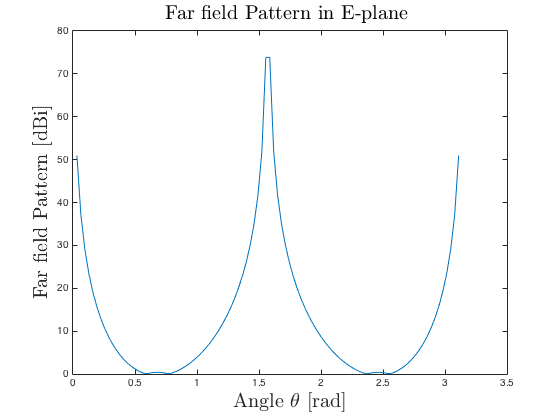
\includegraphics[scale=0.35]{/Users/marikasvensson/Documents/MATLAB/MicroProject/finished/task3/Eplane.png}
\caption{This figure shows the radiation pattern in the E-plane}
\label{task3:E-plane}
\end{figure}


\begin{figure}[h]
\centering
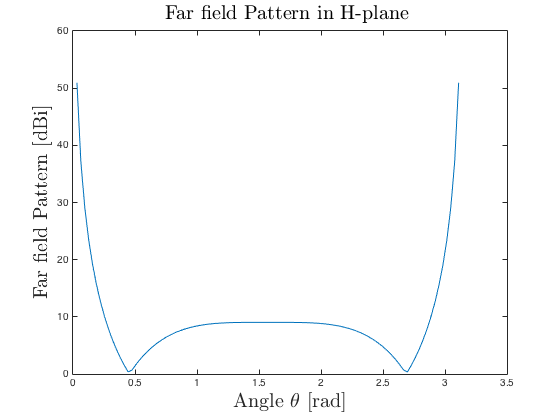
\includegraphics[scale=0.35]{/Users/marikasvensson/Documents/MATLAB/MicroProject/finished/task3/Hplane.png}
\caption{This figure shows the radiation pattern in the H-plane}
\label{task3:H-plane}
\end{figure}

The patterns of the far field function were plotted in figures \ref{task3:PatternE-plane} and \ref{task3:PatternE-plane} for the E- and H-plane. 

\begin{figure}[h]
\centering
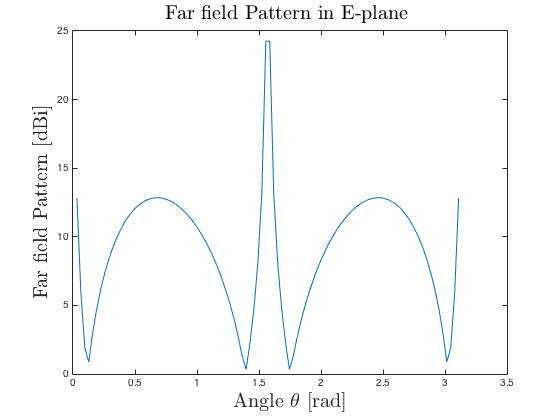
\includegraphics[scale=0.35]{/Users/marikasvensson/Documents/MATLAB/MicroProject/finished/task3/PatternEplane.png}
\caption{This figure shows the far field pattern in the E-plane}
\label{task3:PatternE-plane}
\end{figure}


\begin{figure}[h]
\centering
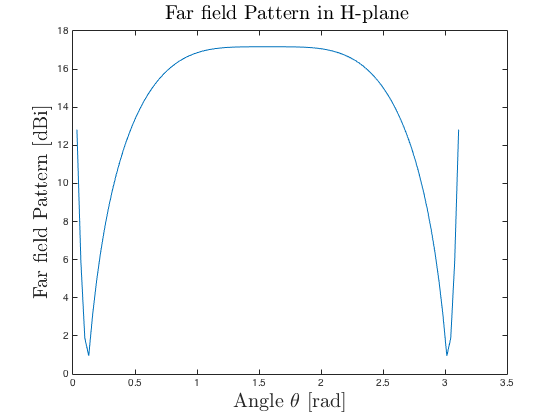
\includegraphics[scale=0.35]{/Users/marikasvensson/Documents/MATLAB/MicroProject/finished/task3/PatternHplane.png}
\caption{This figure shows the far field pattern in the H-plane}
\label{task3:PatternH-plane}
\end{figure}



\chapter{Task 4}
\label{chapter:task4}
In this chapter we began to consider irregular array antennas with N identical elements. Array antennas are good to use as they can for example increase the overall gain, provide diversity reception, steer the array in a particular direction and determine the direction of arrival of the incoming signals.\cite{AntennasFundamentals} 

In this section specifically we were considering an array antenna with irregular spacing $\{\mathbf{r}_i\}_{i=1}^N$ and excitation currents $\{I_i\}_{i=1}^N$. A function was created that takes the positions,  and  excitation vector which gave the far field function of the array antenna as output.
 
\section{Theory}
For antennas with identical elements that lie in an arbitrary array the far field function  may be computed as a sum over the elements in the array elements

\begin{equation}
\mathbf{G}_A(\theta, \phi) = \sum_{n=1}^N A_ne^{j\phi_n}(G_{\theta}\hat{\theta} + G_{\phi}\hat{\phi}) e^{jk\mathbf{r}_n\dot{\hat{r}}}.
\end{equation}
Which can be written as 
\begin{equation}
\mathbf{G}_A(\theta, \phi) = \mathbf{G}(\theta, \phi) \cdot AF
\end{equation}
where AF stands for Array Factor. Further $\mathbf{r}_n$ are the positions of the elements (assumed to be given in $m\lambda$), $A_n$ and $\phi_n$ are the amplitude and phase of the current, respectively. The excitation current can be written in terms of amplitude and phase of the current 
\begin{equation}
\mathbf{I} =[A_1e^{j\Phi_1} A_2e^{j\Phi_2} \dots A_{N-1}e^{j\Phi_{N-1}}],
\end{equation}
it is then easy to compute the far field function. \cite{kildal2000foundations} 

\section{Result}
The MATLAB code for this section can be  viewed in appendix \ref{section:task4.m}. The absolute value of the $\theta$ and $\phi$ parts of the  far field function  were plotted in figures \ref{task4:Gth} and \ref{task4:Gphi} with respect to the angles  $\theta$ and $\phi$, respectively. 

\begin{figure}[h]
\centering
\includegraphics[scale=0.4]{/Users/marikasvensson/Documents/MATLAB/MicroProject/finished/task4/Gth.png}
\caption{This figure shows $G_\theta$ as a function of $\theta$ and $\phi$}
\label{task4:Gth}
\end{figure}


\begin{figure}[h]
\centering
\includegraphics[scale=0.4]{/Users/marikasvensson/Documents/MATLAB/MicroProject/finished/task4/Gphi.png}
\caption{This figure shows $G_\phi$ as a function of $\theta$ and $\phi$}
\label{task4:Gphi}
\end{figure}


\chapter{Task 5}
In this chapter task 4 was continued, the aim was now to attempt to steer the irregular spaced array with an excitation current $I_n  = A_n e^{j\Phi_n}$. This was illustrated by computing a MATLAB function which constructed the excitation current as a function of array antenna positions $\{r_i\}_{i=1}^N$  and steering angles $\theta_0, \phi_0$.

To begin the theory regarding a steered array antenna  and phase shifts will be presented. Then the results from the computations will be presented. 

\section{Theory}
As mentioned before array antennas are good to use because they can be steered, i.e. every element is directed according to a steering vector with fixed angles $\theta_0$ and $\phi_0$. The difference in phase (phase shift) between two elements are $\Phi_{n, n-1}$, which is the length difference of the two elements times the wave vector k. Consider now the spherical coordinates 
\begin{equation}
\hat{r} = sin\theta cos\phi \hat{x} + sin\theta sin\phi \hat{y} + cos\theta \hat{z},
\end{equation}
if the array antenna is steered in a direction $\theta_0$ and $\phi_0$ and the elements of the array are placed in positions $\{\mathbf{r}_i \}_{i=1}^N$ we may project the positions on the steering vector as 
\begin{align}
& d_n = \mathbf{r}_n \cdot \hat{r} = (x_n\hat{x}+ y_n\hat{y} + z_n\hat{z}) (sin\theta_0 cos\phi_0 \hat{x} + sin\theta_0 sin\phi_0 \hat{y} + cos\theta_0 \hat{z})= \\
& sin\theta_0 cos\phi_0 x_n + sin\theta_0 sin\phi_0 y_n + cos\theta_0 z_n.
\end{align}
An illustration of the projection can be viewed in figure \ref{fig:farfieldProjetion}.
\begin{figure}
\centering
\includegraphics[width=0.7\linewidth]{pictures/farfieldProjetion}
\caption{This figure shows how a vector can be projected onto another in the far field region of antennas. This figure was obtained from \cite{kildal2000foundations}}
\label{fig:farfieldProjetion}
\end{figure}
The difference in length between two arbitrary elements in space is thus
\begin{align}
& d_{n,n-1} = |d_n-d_{n-1}| = |\mathbf{r}_n \cdot \hat{r} -\mathbf{r}_{n-1} \cdot \hat{r}| =\\
& | sin\theta_0 cos\phi_0 (x_n -x_{n-1}) + sin\theta_0 sin\phi_0 (y_n -y_{n-1})  + cos\theta_0 (z_n -z_{n-1}) |.
\end{align}
The phase difference  between two elements subsequently  be computed as 
\begin{equation}
\Phi_{n, n-1} = kd_{n,n-1} = \frac{2\pi}{\lambda} | sin\theta_0 cos\phi_0 (x_n -x_{n-1}) + sin\theta_0 sin\phi_0 (y_n -y_{n-1})  + cos\theta_0 (z_n -z_{n-1}) |. 
\end{equation}
However, the actual phase difference that is interesting to compute is the phase difference with respect to the steering vector for each element
\begin{equation}
\Phi_{n, 0} = kd_{n,0} = \frac{2\pi}{\lambda} | sin\theta_0 cos\phi_0 (x_n) + sin\theta_0 sin\phi_0 (y_n)  + cos\theta_0 (z_n)|. 
\end{equation}

It was assumed for this task that the amplitude of the current was 1 A and that the positions are given in $ m \lambda$. Thus the excitation current can be computed to be 
\begin{equation}
I_n = e^{j\Phi_{n, 0}} =e^{ \frac{2\pi}{\lambda} | sin\theta_0 cos\phi_0 (x_n) + sin\theta_0 sin\phi_0 (y_n)  + cos\theta_0 (z_n)| }.
\end{equation}\cite{kildal2000foundations}


\section{Results}
The MATLAB scripts for this section are presented in section \ref{section:task5.m}. The result of the phase of the current was plotted in figure \ref{task5:phase} for an equispaced and irregular array. The amplitude of the current was chosen not to be plotted since the amplitude of the excitation current was assumed to be unity.

\begin{figure}[h]
\centering
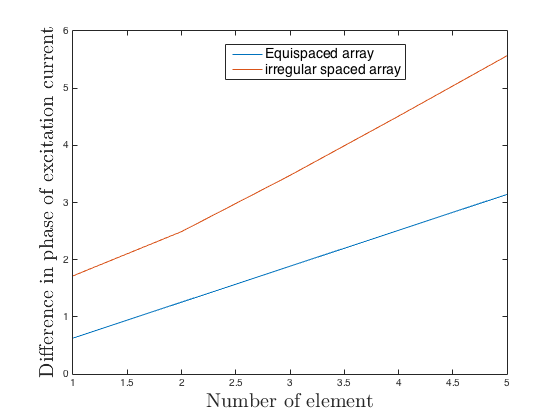
\includegraphics[scale=0.6]{/Users/marikasvensson/Documents/MATLAB/MicroProject/finished/task5/excitationCurrent.png}
\caption{This figure shows the phase with respect to the steering vector of the excitation current as a function of element positions and steering direction $\theta_0 = \pi/3$rad and $\phi_0 = \pi/2$rad }
\label{task5:phase}
\end{figure}

The phase difference between the elements were also computed an plotted in figure \ref{task5:phaseNeigh}.

\begin{figure}[h]
\centering
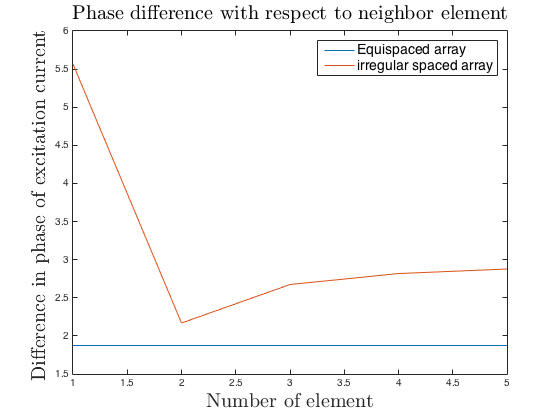
\includegraphics[scale=0.6]{/Users/marikasvensson/Documents/MATLAB/MicroProject/finished/task5/excitationCurrentNeighbour.png}
\caption{This figure shows the phase of the excitation current with respect to the neighbor as a function of element positions and steering direction $\theta_0 = \pi/3$rad and $\phi_0 = \pi/2$rad }
\label{task5:phaseNeigh}
\end{figure}




\begin{comment}
\begin{equation}
\Psi_n = \frac{2\pi}{\lambda}( d_n sin(\theta_0) )
\end{equation}
where $\theta_0$ is the scanning angle and $\d_n = |\mathbf{r}_n - \mathbf{r}_{n-1}|$ is the intermediate distance between element n and n-1. 



The total phase shift for an element should then be 
\begin{equation}
\phi_n^{tot} = \sum_{i=1}^n \Psi_i.
\end{equation} 
% Calculatin the amplitude??
For the amplitude we may use the formula we will set the current amplitude to 1. 





A steering vector $\mathbf{v(k)}$ is the representation of the phase delay that each element in the array antenna has, which is defined as 

\begin{equation}
\mathbf{v(k)}=[e^{-j\mathbf{k}\cdot\mathbf{r}_1} ... e^{-j\mathbf{k}\cdot\mathbf{r}_N} ]
\end{equation}
We can write an output function Y as 

\begin{equation}
R_A = R(\theta, \phi) \sum_i w_ie^{-j\mathbf{k}\cdot\mathbf{r}_i} = G(\theta, \phi)AF
\end{equation}
where

\begin{equation}
AF = \mathbb{w}^T\mathbf{v(k)}
\end{equation}
and  $R(\theta, \phi)$
\if
\end{comment}

\chapter{Task 6}
\label{chapter:task6}
An N dimensional equispaced array antenna  with identical elements was considered in this section. Having an equispaced array antenna simplifies the computations as we know that the phase difference between the elements will be the same for every element (i.e. constant phase difference).

The positions, $\{\mathbf{r}_n\}_{i=1}^N$, of the antennas can be written as  
\begin{equation}
\mathbf{r}_n = \mathbf{r}_c + a_n \hat{a} = \mathbf{r}_c + \left (n + \frac{N+1}{2}\right)d\hat{a}
\end{equation}
where $\mathbf{r}_c$ is the center of the array and we have intermediate  spacing d the total length is then Nd and we may write the electrical field as 
\begin{equation}
\mathbf{E}_n(\mathbf{r}) = \frac{e^{-jkr}}{r} \mathbf{G}(\mathbf{r}).
\end{equation}
We have earlier defined the far field function and the array  factor in section \ref{chapter:task4}, which now allows us to consider the array factors and the radiation patterns. If the antenna is directed at an angle $\theta$  the array factor can be written as 
\begin{align}
&AF = 1 + e^{j(kd\cdot 1 cos(\theta) +\alpha)}  + ... + e^{j\cdot(N-1)(kdcos(\theta) +\alpha)} = \\ & \sum_{n=1}^N  e^{j(kd\cdot (n-1)) cos(\theta) +\alpha)} = e^{j(N-1)\Psi/2}sin(N\Psi/2)/ sin(\Psi/2)
\end{align}
where $\Psi = \alpha + kdcos(\theta)$ and assuming that the elements of the antenna are equal.

\section{Task 6 a}
In this section the array antenna with 5 elements was considered for intermediate element spacing $d = \lambda/4$ pointed in the H-plane. Firstly the theory regarding the array antennas and the H-plane will be presented. Then the results from the MATLAB simulations will be presented. 
\subsection{Theory}
The total radiation pattern of an array antenna is defined as  
\begin{equation}
Pattern_{radiation}^{tot} = (\text{element radiation pattern})\times(AF).
\end{equation}
 For an equispaced array with intermediate spacing d and N-1 elements there will be a phase difference $\alpha$ between every element. The normalized array factor can the be written as 
\begin{equation}
|AF| = sin(N\Psi/2)/( N sin(\Psi/2) ).
\end{equation}
where $\Psi = \alpha + kdcos\theta$.  As we are considering horizontal dipole antennas the radiation pattern in the far field region will be 
\begin{equation}
f = \sqrt{1-sin^2(\theta)cos^2(\phi)}
\end{equation}
A maximum of the array factor can be found at $\Psi$ =0 which corresponds to $\alpha = kdcos(\theta_0)$ where $\theta_0$ is called the steering angle. This will simplify the expression when the array antenna is directed at a specific region. The radiation patterns the total radiation pattern can thus be plotted in the H plane  which corresponds with $\alpha = kdcos(\theta_0) =kd$, i.e. $\theta_0 =0$\cite{AntennasFundamentals}. \cite{kildal2000foundations}

The radiation pattern, far field pattern may be normalized and plotted in dBi as described in chapter \ref{chapter:task3}.

\subsection{Results}
The MATLAB scripts for the simulation if the H-plane can be viewed in appendix \ref{section:task6a.m}. The plotted results for  the radiation-, far field- and AF-patterns were plotted in figures \ref{task6a:ypol}, \ref{task6a:ypolHpat} and \ref{task6a:ypolAF}, respectively. 

\begin{figure}[h]
\centering
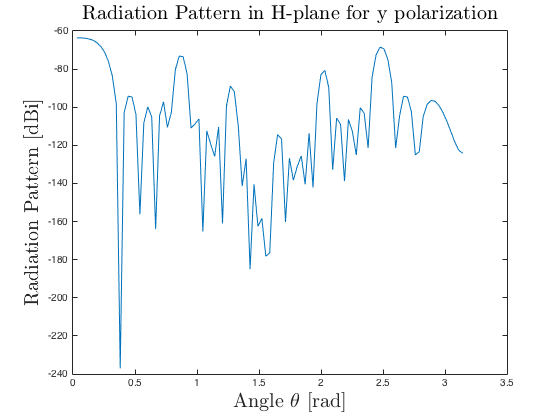
\includegraphics[scale=0.4]{/Users/marikasvensson/Documents/MATLAB/MicroProject/finished/task6/6a/ypolHplane.png}
\caption{This figure shows the radiation pattern as a function of $\theta$in the H-plane}
\label{task6a:ypol}
\end{figure}

\begin{figure}[h]
\centering
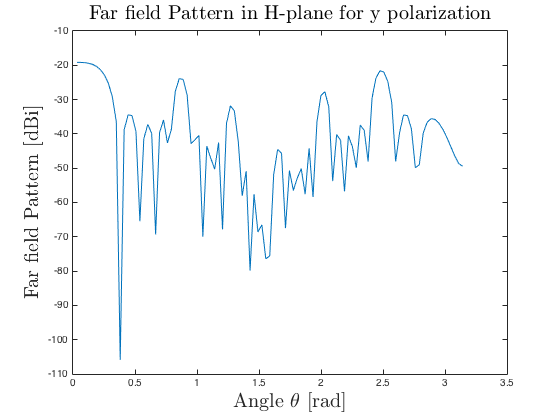
\includegraphics[scale=0.4]{/Users/marikasvensson/Documents/MATLAB/MicroProject/finished/task6/6a/ypolHplanePattern.png}
\caption{This figure shows the far field pattern as a function of $\theta$in the H-plane}
\label{task6a:ypolHpat}
\end{figure}

\begin{figure}[h]
\centering
\includegraphics[scale=0.4]{/Users/marikasvensson/Documents/MATLAB/MicroProject/finished/task6/6a/ypolAF.png}
\caption{This figure shows $AF$ as a function of $\theta$ and $\phi$ for y polarized dipoles}
\label{task6a:ypolAF}
\end{figure}
\FloatBarrier

\section{Task 6 b}
In this section the array antenna with 5 elements was considered for intermediate element spacing $d \in \lambda[1/4,4]$ pointed in the broadside direction. Firstly the theory regarding the array antennas and the broadside will be presented. Then the results from the MATLAB simulations will be presented. 
\subsection{Theory}
Consider the theory in task 6a, this is  the theory which is needed to compute the  result here as well but with some small adjustments. 
The radiation patterns the total radiation pattern can be plotted in the broadside, this corresponds with $\alpha = kdcos(\theta_0) = 0 $. The steering angle is thus $\theta_0 = \pi/2$. \cite{kildal2000foundations}

\subsection{Results}
The MATLAB scripts for the simulation if the H-plane can be viewed in appendix \ref{section:task6a.m}. The plotted results for  the radiation- , far field- and AF-patterns were plotted in figures \ref{task6b:ypol}, \ref{task6b:ypolHpat} and \ref{task6b:ypolAF}, respectively. The figures illustrates the radiation pattern for d $\in \lambda[1/4, 4].$ 

\begin{figure}[h]
\centering
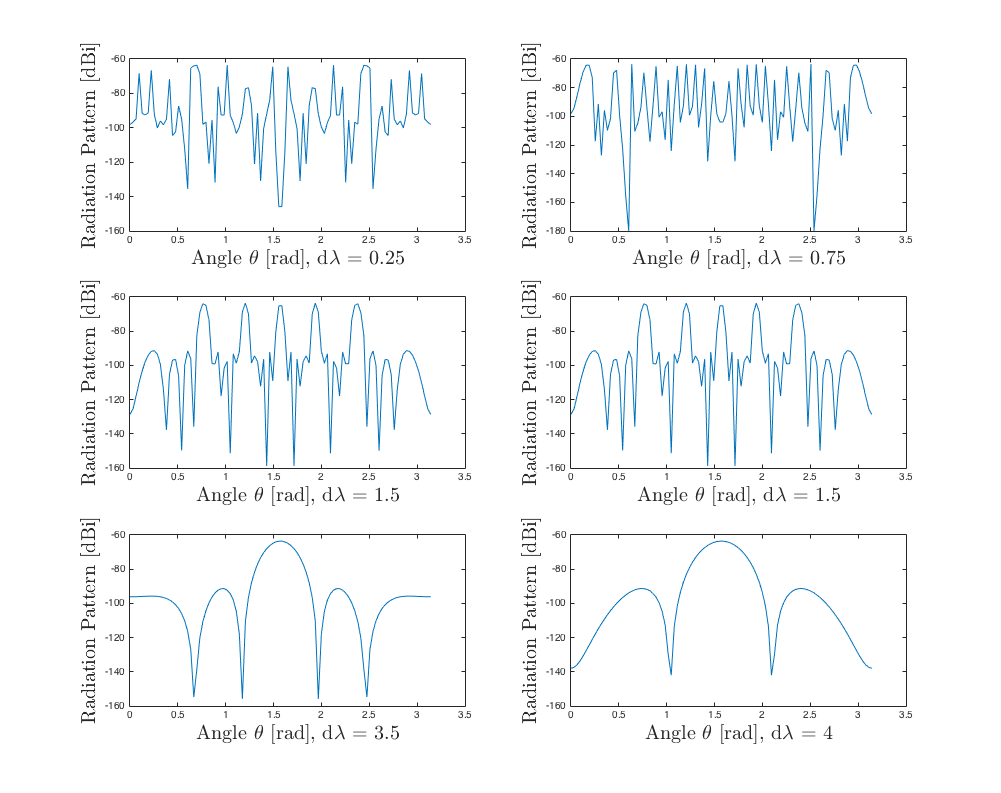
\includegraphics[scale=0.5]{/Users/marikasvensson/Documents/MATLAB/MicroProject/finished/task6/6b/ypolbroad.png}
\caption{This figure shows the radiation pattern as a function of $\theta$ for y polarized dipoles in an array}
\label{task6b:ypol}
\end{figure}

\begin{figure}[h]
\centering
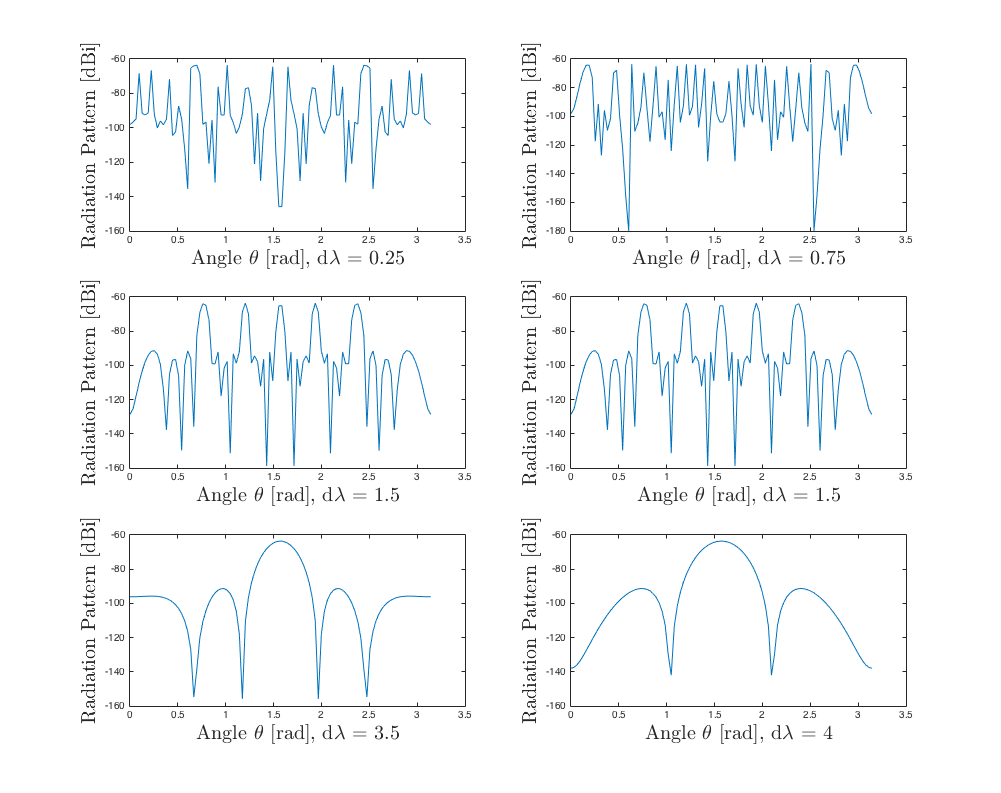
\includegraphics[scale=0.5]{/Users/marikasvensson/Documents/MATLAB/MicroProject/finished/task6/6b/ypolbroad.png}
\caption{This figure shows the far field pattern as a function of $\theta$ for y polarized dipoles in arrays}
\label{task6b:ypolHpat}
\end{figure}

\begin{figure}[h]
\centering
\includegraphics[scale=0.5]{/Users/marikasvensson/Documents/MATLAB/MicroProject/finished/task6/6b/ypolAF.png}
\caption{This figure shows $AF$ as a function of $\theta$ and $\phi$ for y polarized dipoles}
\label{task6b:ypolAF}
\end{figure}



 \chapter{Discussion and conclusion}
 \label{chapter:discussion}
 

 %Task1: Compare  expectations and our results
 In the first task the different parts of the far field function could be viewed in the plots, I have not found any reference for this function yet, but it appear to correspond to the analytical expression. Thus the conclusion is that the MATLAB function works correctly. 
 
 
 %Task 2: Compare  expectations and our results
 In task 2 the result of the total radiation the result gave the same for every polarization, as expected. 
 
 
In task 3 the patterns of the far field function were plotted when normalized with respect to the total radiated power in the E- and H-plane. These patterns do resemble the expected result.
 
 
 
 In the fourth task the different parts of the far field function could be viewed in the plots for a given current I, as a arbitrary current was chosen it was somewhat difficult to analyze the result. The result resembles the result in task 1 somewhat. Thus the conclusion is that the MATLAB function works correctly.
 
%Task5:  Compare  expectations and our results
In task 5 it can be noted that the MATLAB function gives the expected phase difference for the equispaced 
 array as the phase linearly increases with the distance from the origin. Simultaneously the phase difference between the individual neighbor elements remained constant through out the array. 
 
 In task 6 the patterns are quite symmetric, which was expected. Giving the conclusion that the MATLAB function is correct. 

\appendix

\chapter{Source code}

\section{Task 1}
\label{section:task1.m}

\subsection{\texttt{Task1.m}}
\lstinputlisting[language=matlab,numbers=left]{/Users/marikasvensson/Documents/MATLAB/MicroProject/finished/task1/task1.m}


\subsection{\texttt{horizontalDipole.m}}
\lstinputlisting[language=matlab,numbers=left]{/Users/marikasvensson/Documents/MATLAB/MicroProject/finished/task1/horizontalDipole.m}



\section{Task 2}
\label{section:task2.m}
\subsection{\texttt{Task2.m}}
\lstinputlisting[language=matlab,numbers=left]{/Users/marikasvensson/Documents/MATLAB/MicroProject/finished/task2/task2.m}


\subsection{\texttt{totalPwr.m}}
\lstinputlisting[language=matlab,numbers=left]{/Users/marikasvensson/Documents/MATLAB/MicroProject/finished/task2/totalPwr.m}


\section{Task 3}
\label{section:task3.m}
\subsection{\texttt{Task3.m}}
\lstinputlisting[language=matlab,numbers=left]{/Users/marikasvensson/Documents/MATLAB/MicroProject/finished/task3/task3.m}


\subsection{\texttt{totalPwr.m}}
\lstinputlisting[language=matlab,numbers=left]{/Users/marikasvensson/Documents/MATLAB/MicroProject/finished/task3/totalPwr.m}


\section{Task 4}
\label{section:task4.m}

\subsection{\texttt{Task4.m}}
\lstinputlisting[language=matlab,numbers=left]{/Users/marikasvensson/Documents/MATLAB/MicroProject/finished/task4/task4.m}


\subsection{\texttt{totalPwr.m}}
\lstinputlisting[language=matlab,numbers=left]{/Users/marikasvensson/Documents/MATLAB/MicroProject/finished/task4/compGfromAandI.m}


\section{Task 5}
\label{section:task5.m}

\subsection{\texttt{Task5.m}}
\lstinputlisting[language=matlab,numbers=left]{/Users/marikasvensson/Documents/MATLAB/MicroProject/finished/task5/task5.m}


\subsection{\texttt{excitationVector.m}}
\lstinputlisting[language=matlab,numbers=left]{/Users/marikasvensson/Documents/MATLAB/MicroProject/finished/task5/excitationVector.m}

\subsection{\texttt{excitationVector1.m}}
\lstinputlisting[language=matlab,numbers=left]{/Users/marikasvensson/Documents/MATLAB/MicroProject/finished/task5/excitationVector1.m}





\section{Task 6}


\subsection{\texttt{Task6\_a.m}}
\label{section:task6a.m}
\lstinputlisting[language=matlab,numbers=left]{/Users/marikasvensson/Documents/MATLAB/MicroProject/finished/task6/task6_a.m}


\subsection{\texttt{Task6\_b.m}}
\label{section:task6b.m}
\lstinputlisting[language=matlab,numbers=left]{/Users/marikasvensson/Documents/MATLAB/MicroProject/finished/task6/task6_b.m}


\subsection{\texttt{totalPwr.m}}
\lstinputlisting[language=matlab,numbers=left]{/Users/marikasvensson/Documents/MATLAB/MicroProject/finished/task6/totalPwr.m}

\bibliographystyle{IEEEtran}
\bibliography{IEEEabrv,refs}
%\bibliographystyle{plain}
%\bibliography{refs}
\end{document}


http://www.antenna-theory.com/

http://www.kyes.com/antenna/navy/freq-phase/freqphas.htm

http://www.ece.mcmaster.ca/faculty/nikolova/antenna_dload/current_lectures/L13_Arrays1.pdf


http://www.diva-portal.org/smash/get/diva2:211543/FULLTEXT02.pdf


http://www.ece.rutgers.edu/~orfanidi/ewa/